\chapter*{Introduction}
\addcontentsline{toc}{chapter}{Introduction}
%
\linenumbers
%
Modern society is facing huge challenges. Climate change and the need for cleaner energy to reduc green-house gas emissions, clashing with the hope of permanent economic growth and global exchange of information, goods and people. Unprecedented issues arise from this more and more technologically advanced and interconnected civilization. This PhD work was initiated in the middle of the most impactful sanitary crisis of the contemporary era, the COVID-19 pandemic. 
Deep ultraviolet is a radiation that kills the coronavirus. (Show market share of UV emitters and applications)
Moreover, technological innovation could bring a way to produce cleaner energy, such as fusion which is a priority research topic, or photovoltaic, but also energy storage, preferably without the need to extract rare materials. Effort should be put into the use of sustainable and abundant base material.
Importance of theoretical estimation of the capabilities of certain materials for optoelectronic devices fabrication (check intro of Kioupakis talk at EPFL)
hBN is promising for its properties and is not rare
miniaturization of devices brings more attention towards heterostructures whose building blocks are single-atom-thick layers. With the variety of optical and electronic properties offered by all the existing monolayers, and the engineering of their stacking, twisting, and straining as well as their interaction with substrates, the possibilities for devices are almost limitless. In this ecosystem, hexagonal Boron Nitride is a candidate of choice for its structural, electronic and optical properties.

The 2020 UV emitter roadmap : Hiroshi Amano et al 2020 J. Phys. D: Appl. Phys. 53 503001
UV to kill coronavirus : https://doi.org/10.1016/j.jphotobiol.2020.112044
Hsu, Tsung-Chi, et al. "Perspectives on UVC LED: Its progress and application." Photonics. Vol. 8. No. 6. MDPI, 2021.
In 2019, the total market for UV LEDs reached US\$ 144M,mostly driven by water disinfection. Following the COVID-19 outbreak, demand for UVGI greatly increased, and a five-fold growth in surface disinfection applications has been predicted by Yole Développement, leading to a total UV LED market of up to US\$ 300M 
% cite : Yole-Developpement 2020UVC LEDs : One Solution toContain the COVID-19 Pandemic(available at:http://www.yole.fr/iso_upload/News/2020/PR_UV_LED_MarketUpdate_YOLEGROUP_Oct2020.pdf)

%
Optical measurements are an efficient way to characterize materials and reveal the microscopic (quantum) interplay between electronic wavefunctions and electromagnetic field of light, and collective quantum effects in the crystal (plasmons, excitons, etc)
%
process of optical excitation ; what is a hole ; describe indirect transitions, assisted with phonons

differences absorption vs luminescence : in hBN two different exciton states dominate the two processes
%
%
HPC is crucial
%

electronic and optical properties of layered materials (an in particular BN) can be modified by many factors
strain \cite{blundo2021strain}, stacking (cite sponza2018direct), twisted angle (cite latil2023structural, impellizzeri2022electronic), substrate interaction etc...\\


Generalities about hBN \\
AA'-hBN is stable at room temperature and ambient pressure
hBN : hig gap, pDOS of valence at K is mostly Nitrogen, $\pi$ orbital(overlap of $p_z$, bonding)  . pDOS of conduction at M is mostly Boron, $\pi^*$ orbital (overlap of $p_z$ with opposite coefficient, antibonding)\\
%We could compute phonon-assisted absorption but the phonon satellites are very small wrt to the main peaks so when they overlap, they are not visible.\\

In condensed matter, the problem of exciton-phonon coupling and phonon-assisted luminescence is an old topic. The first studies date back to the 60s by Toyozawa \emph{et al.}\cite{toyozawa2003optical,toyozawa1964interband} and the first dynamical solution of the Bethe-Salpeter equation (BSE), the so-called Shindo solution, was proposed precisely to study the exciton-phonon problem.\cite{shindo1970effective}
More recently, this problem has been studied in different materials, from nanotubes\cite{perebeinos} to 2D crystals, and new methodologies were introduced, such as the cumulant Ansatz\cite{cudazzo2020first}, polaron transformation,\cite{feldtmann2009phonon} density matrix,\cite{brem2020phonon} two-particles Green's functions\cite{antonius2017theory} and real-time approach,\cite{paleari2022coupling} with the aim of deriving a modern formulation of exciton-phonon interaction and its related observables, such as phonon-assisted luminescence, within many-body perturbation theory (MBPT).

Theory of phonon-assisted optics : it exists. For instance, Williams-Lax theory that treats lattice-dependent band features and phonon-assisted transitions 
There is also Hallen-Bardeen-Blatt and Heine-Cardona but I don't know too much about them.
Besides, some models of exciton-phonon coupling exists also, some specifically for luminescence, but they are computationally expensive for real materials.
Zacharias and Giustino (+ Jordan?) derive a formalism based on Williams-Lax to describe phonon-assisted absorption 

==> there is a need for exciton-phonon coupling and phonon-assisted optics from first principles. In Chapters 2 and 3, two different approaches are presented in Sections \ref{sec:excph_fdd} and \ref{sec:excph_ai}. The first one consists in calculating the response function correction due to exciton-phonon coupling from finite differences, by displacing atoms in supercells. The second one is a more general approach based on \acrshort{MBPT}, in which a dynamical correction induced by electron-phonon coupling is added as a perturbation to the static Bethe-Salpeter kernel. Thanks to this \textit{ab initio} framework, the scattering of every exciton with every phonon mode can be computed, over the whole Brillouin Zone. These calculations are done in the unit cell.
Both approaches allow to compute the exciton-phonon coupling. Then, the absorption can be obtained after post-processing of a standard \acrshort{BSE} calculation. To obtain the luminescence spectra, we use the van Roosbroeck -- Shockley relation for both cases.
Exciton-phonon in hBN are not only possible, but likely due to strong electron-phonon coupling. Verified experimentally by the External Quantum Efficiency comparable to direct gap materials.\\
\begin{figure}[h!b]
	\vspace{0.2cm}
	\setcapindent{2em}
	\centering
	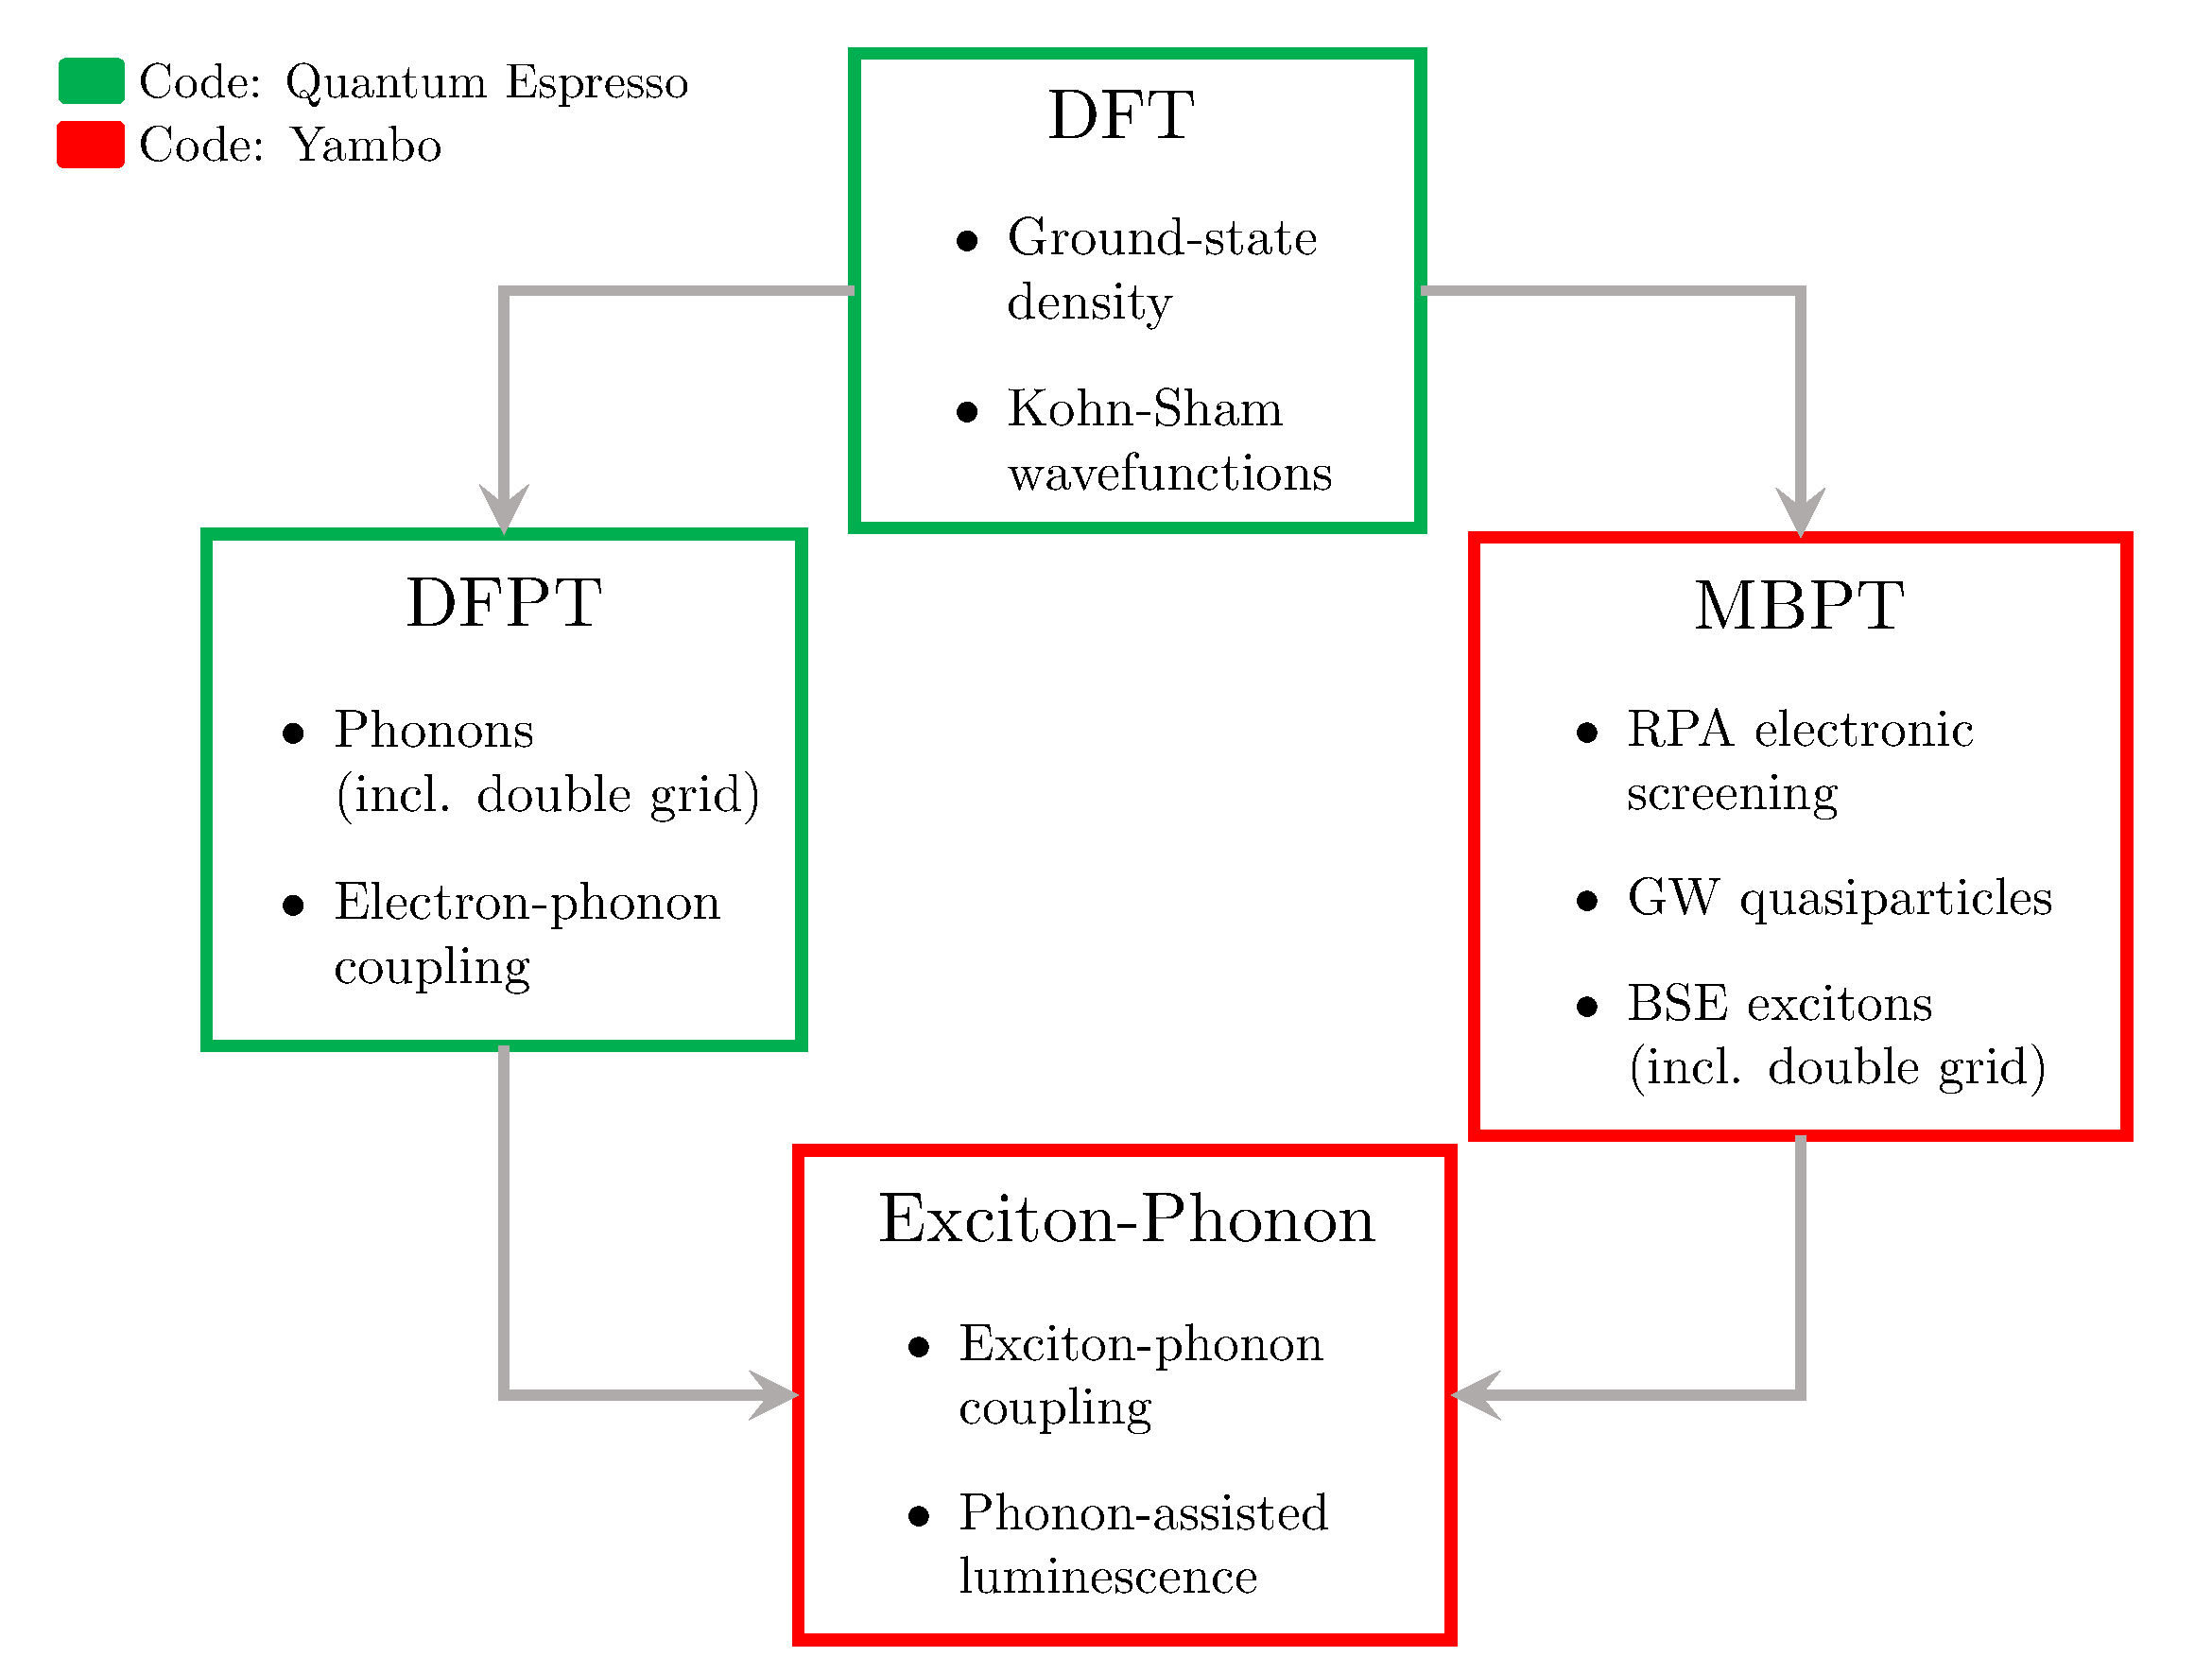
\includegraphics[width=0.9\textwidth]{workflow_detailed.pdf}
	\caption{Workflow of the calculations to compute exciton-phonon coupling and phonon-assisted luminescence. The green/red boxes indicate that we used \textsc{Quantum ESPRESSO} / \yambo~as simulation codes.}
	\label{fig:workflow}
\end{figure}



%
Chapter 1 introduces the theoretical framework in which our calculations are contained. It includes a brief description of the widely used \acrfull{DFT}. In this theory the electrons are treated as independent particles evolving in a mean-field. It allows to compute the ground state density of the crystal and to obtain the equilibrium geometries, with a certain set of approximations. From there we extract the Kohn-Sham eigenvalues and wavefunctions. These eigenvalues give an approximation to the band structure and are the starting point of the more involved \acrfull{MBPT}. 

\acrshort{MBPT} is based on Green's functions and treats the many-body interactions as a perturbation of the independent-particle system. The main equations of this theory are the Hedin's equations, whose derivation is sketched in this first Chapter. Truncating this set of self-consistent equations by neglecting the electron-hole interaction gives the $GW$ approximation. This is an improvement with respect to \acrshort{DFT} in the sense that the electrons are now dressed with the interactions with surrounding electrons. They become \textit{quasiparticles}, whose evolution in time and space is easier to describe. With this we are able to obtain a more accurate band structure and simulate experiments that involve charged excitations. However the neutral excitations of the many-electron system are not well described at this point. To this end, the electron-hole interaction is reintroduced by computing the two-particle Green's function. This is the solution of the so-called \acrfull{BSE}. Starting from the $GW$ approximation, the \acrshort{BSE} can be formulated in the basis of \textit{excitons}, which are quasiparticles made of a bound electron-hole pair. From the \acrshort{BSE} one can obtain the response function of the system including excitonic effects, with the assumption that excitations are instantaneous in time and response to these excitations. This is known as the \textit{static} approximation. Excitons have been shown to play a significant role in the optical spectra of \acrshort{hBN} and indeed the \acrshort{BSE} description is in much better agreement with experiments compared to independent-particles or quasiparticles levels of theory, as can be seen in Fig. \textcolor{red}{Figure of absorption}. The link between microscopic excitonic quantities and macroscopic observables is presented in the middle of the first Chapter. 

Then, we present a perturbative method based on \acrshort{DFT} to obtain the vibrational properties of the crystal in the harmonic approximation, meaning that each atom is represented as an harmonic oscillator vibrating around its equilibrium position. It is called \acrfull{DFPT}. In second quantization, it gives a description of the vibration modes of the lattice in terms of quanta of vibration called \textit{phonons}. They are another type of quasiparticle with a definite frequency and wave vector, analogous to the crystal momentum of electrons. 


\textcolor{blue}{\texttt{GW : dynamical screening ; BSE : static screening}}

at the end of the description of chapter , put the workflow
after the workflow, talk about the way we compute excph coupling in the two Chapters

describe chapter 2
describe chapter 3
appendices
% ETSF webinar of Fulvio
% indirect bandgap only; we can write the response function with derivatives of the response function because we consider only phonon-assisted transitions; need supercells
% PLE (propto absorption) or absorption and PL are not symmetric, as expected for direct gaps
% the minimum exciton at T is the degenerate dark state at Gamma which splits
% for absorption, the bright exciton overlaps with the phonon replicas and it is so bright that we don't see them 

